%% 第3章 AI Agent 智能体编排系统概要设计

\chapter{AI Agent 智能体编排系统概要设计}

\section{系统结构设计}

系统采用\textbf{领域驱动设计（DDD）的分层架构}和前后端分离的部署模式，
后端分为接口层、应用层、领域层、基础设施层四个 Maven 子模块，
前端基于 React + TypeScript 实现。系统整体结构如图~\ref{fig:sys_struct}~所示。

\begin{figure}[H]
  \centering
  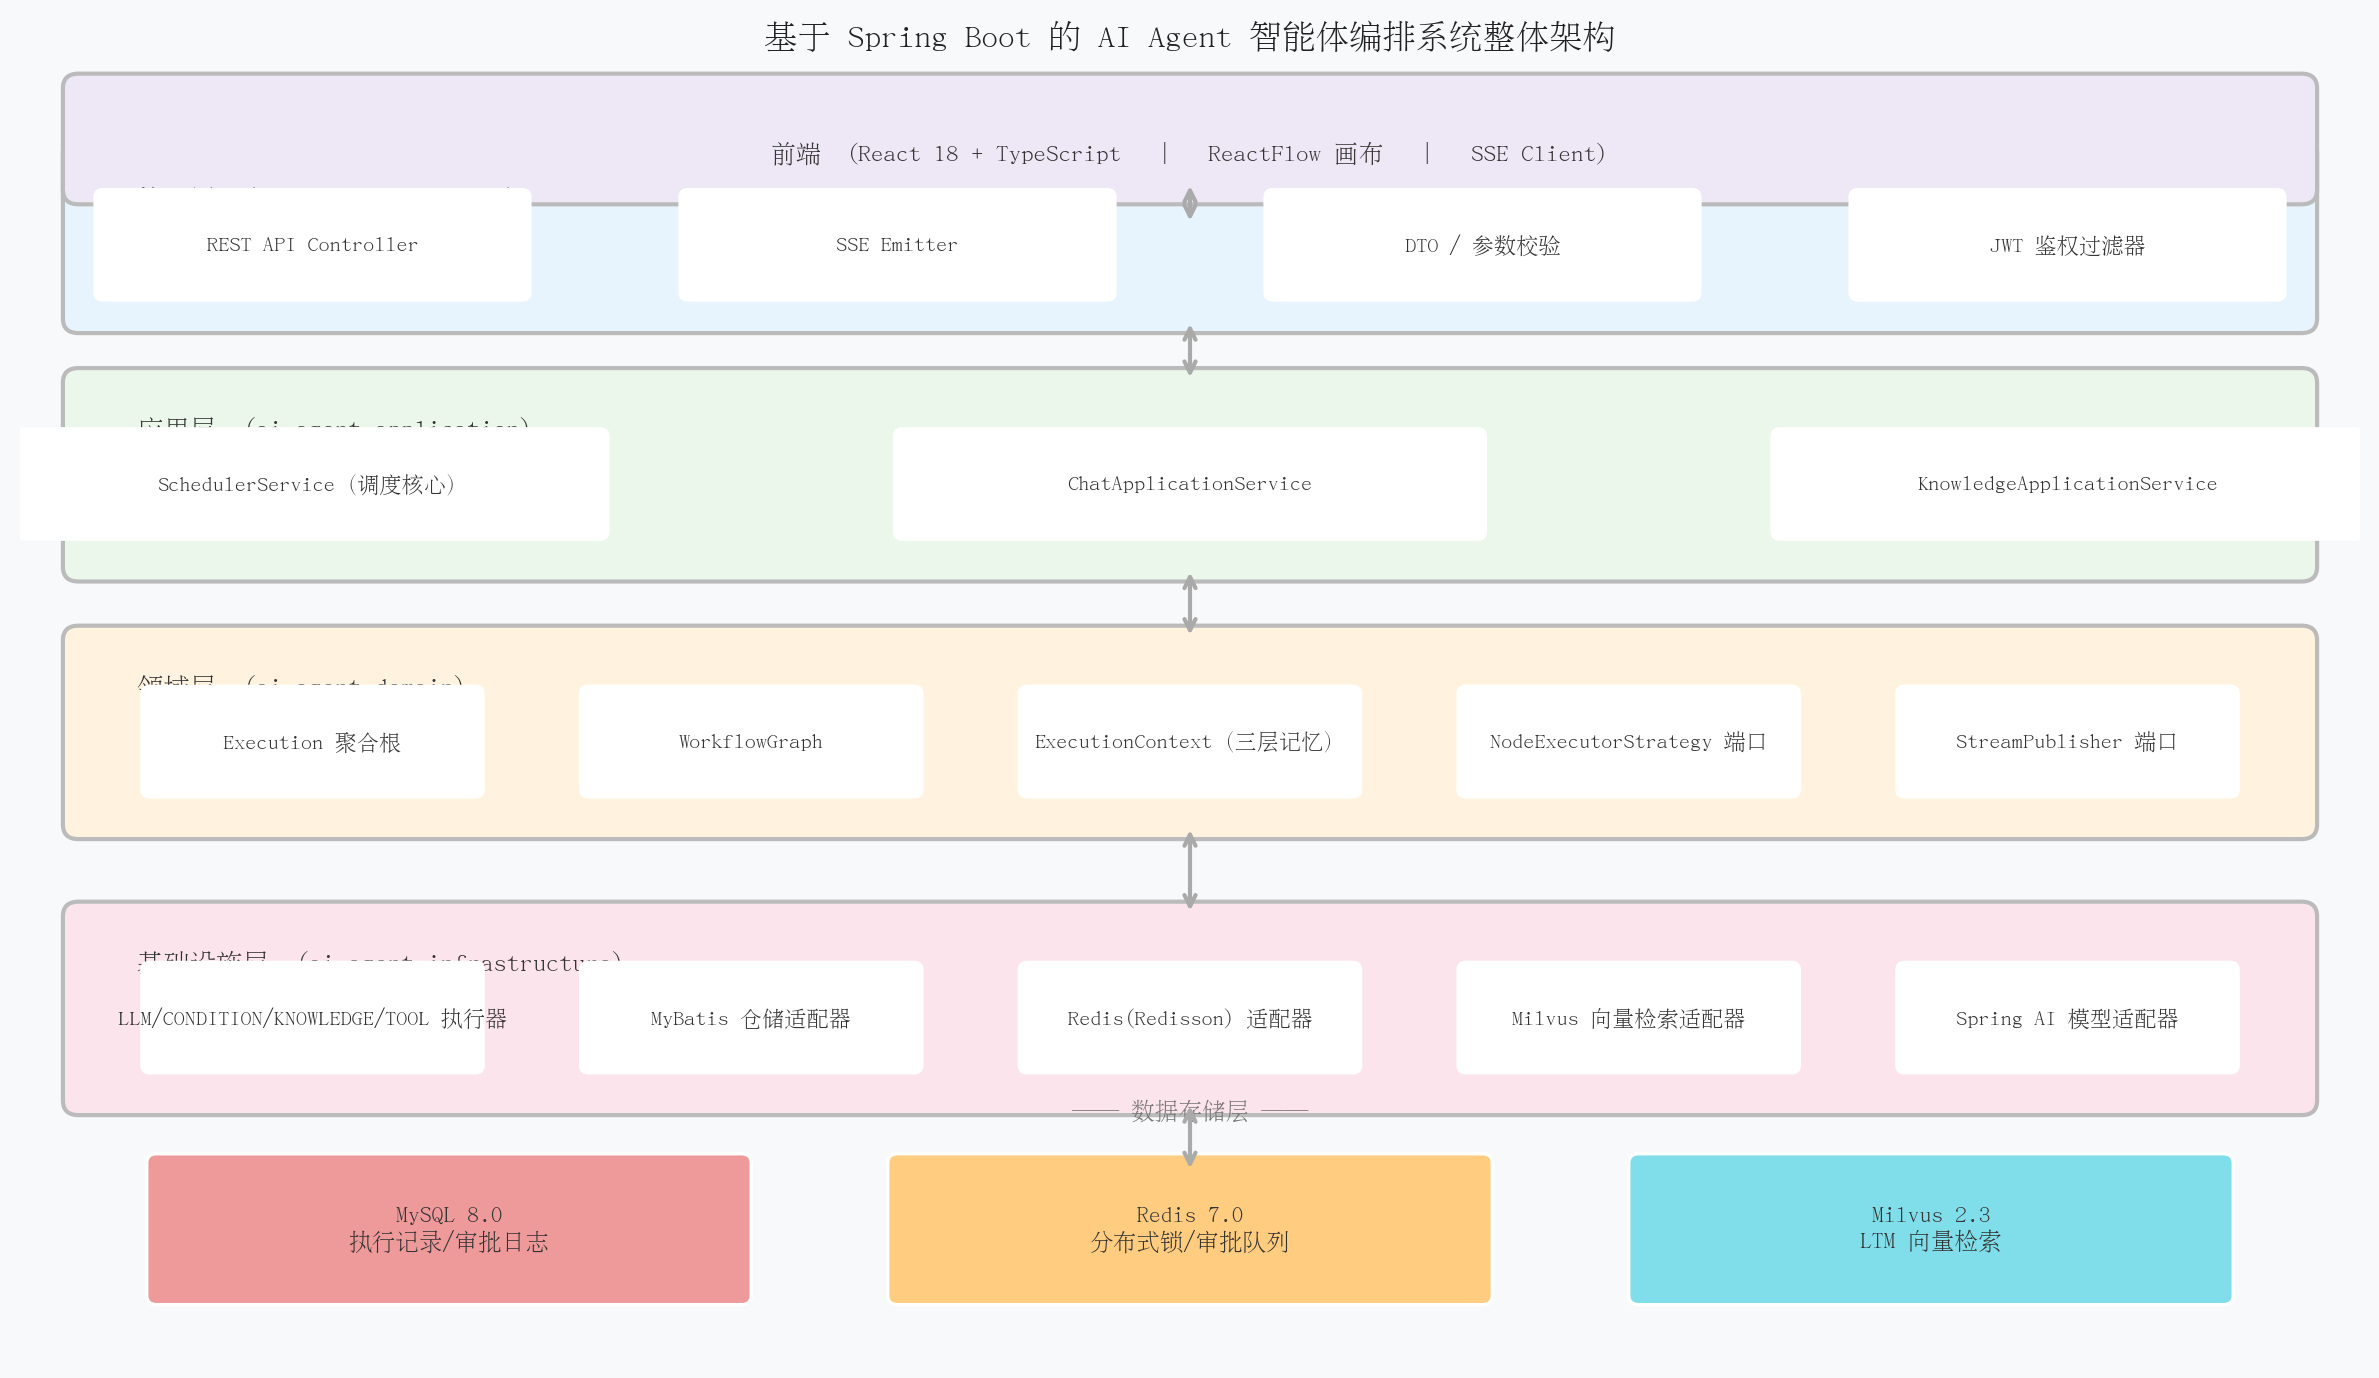
\includegraphics[width=0.95\textwidth]{figures/fig_arch.png}
  \caption{系统整体结构图}
  \label{fig:sys_struct}
\end{figure}

各层的技术组成和核心职责如下：

\textbf{接口层（ai-agent-interfaces）：}
提供 RESTful API 控制器（Controller），负责处理 HTTP 请求、参数校验、
DTO 与领域对象的转换，以及 SSE 连接的建立与维护。
用户注册、登录、知识库管理、审批接口和工作流启动接口均在此层对外暴露。

\textbf{应用层（ai-agent-application）：}
包含 Agent 管理服务、工作流调度服务、知识应用服务和用户应用服务等。
该层负责跨聚合编排，例如协调 Agent 查询、工作流 DAG 解析、知识检索增强、
审批恢复与异步文档处理等，但不承载具体领域规则本身。

\textbf{领域层（ai-agent-domain）：}
系统业务逻辑的核心，包含 \texttt{Execution} 聚合根（DAG 状态流转）、
\texttt{WorkflowGraph}（图结构）、\texttt{KnowledgeDocument}、\texttt{User} 等核心领域对象，
以及向量检索、文件存储、文本切分、邮件服务等端口接口。
领域层保持纯净，不依赖任何框架或外部库。

\textbf{基础设施层（ai-agent-infrastructure）：}
实现领域层定义的端口接口，包括节点执行器策略（LLM/CONDITION/KNOWLEDGE/TOOL/START/END）、
MySQL 仓储适配器、Redis 客户端、Milvus 向量存储适配器、MinIO 文件存储适配器、
邮件发送实现以及 Spring AI 模型适配器。

前端（ai-agent-forward）基于 React + TypeScript 实现，
包含 Agent 列表与画布编排页、对话执行页、人工审批页、知识库页和登录注册页等功能页面。

\section{系统功能设计}

根据需求分析，系统围绕五个核心模块展开设计，功能结构如图~\ref{fig:func_struct}~所示。

\begin{figure}[H]
  \centering
  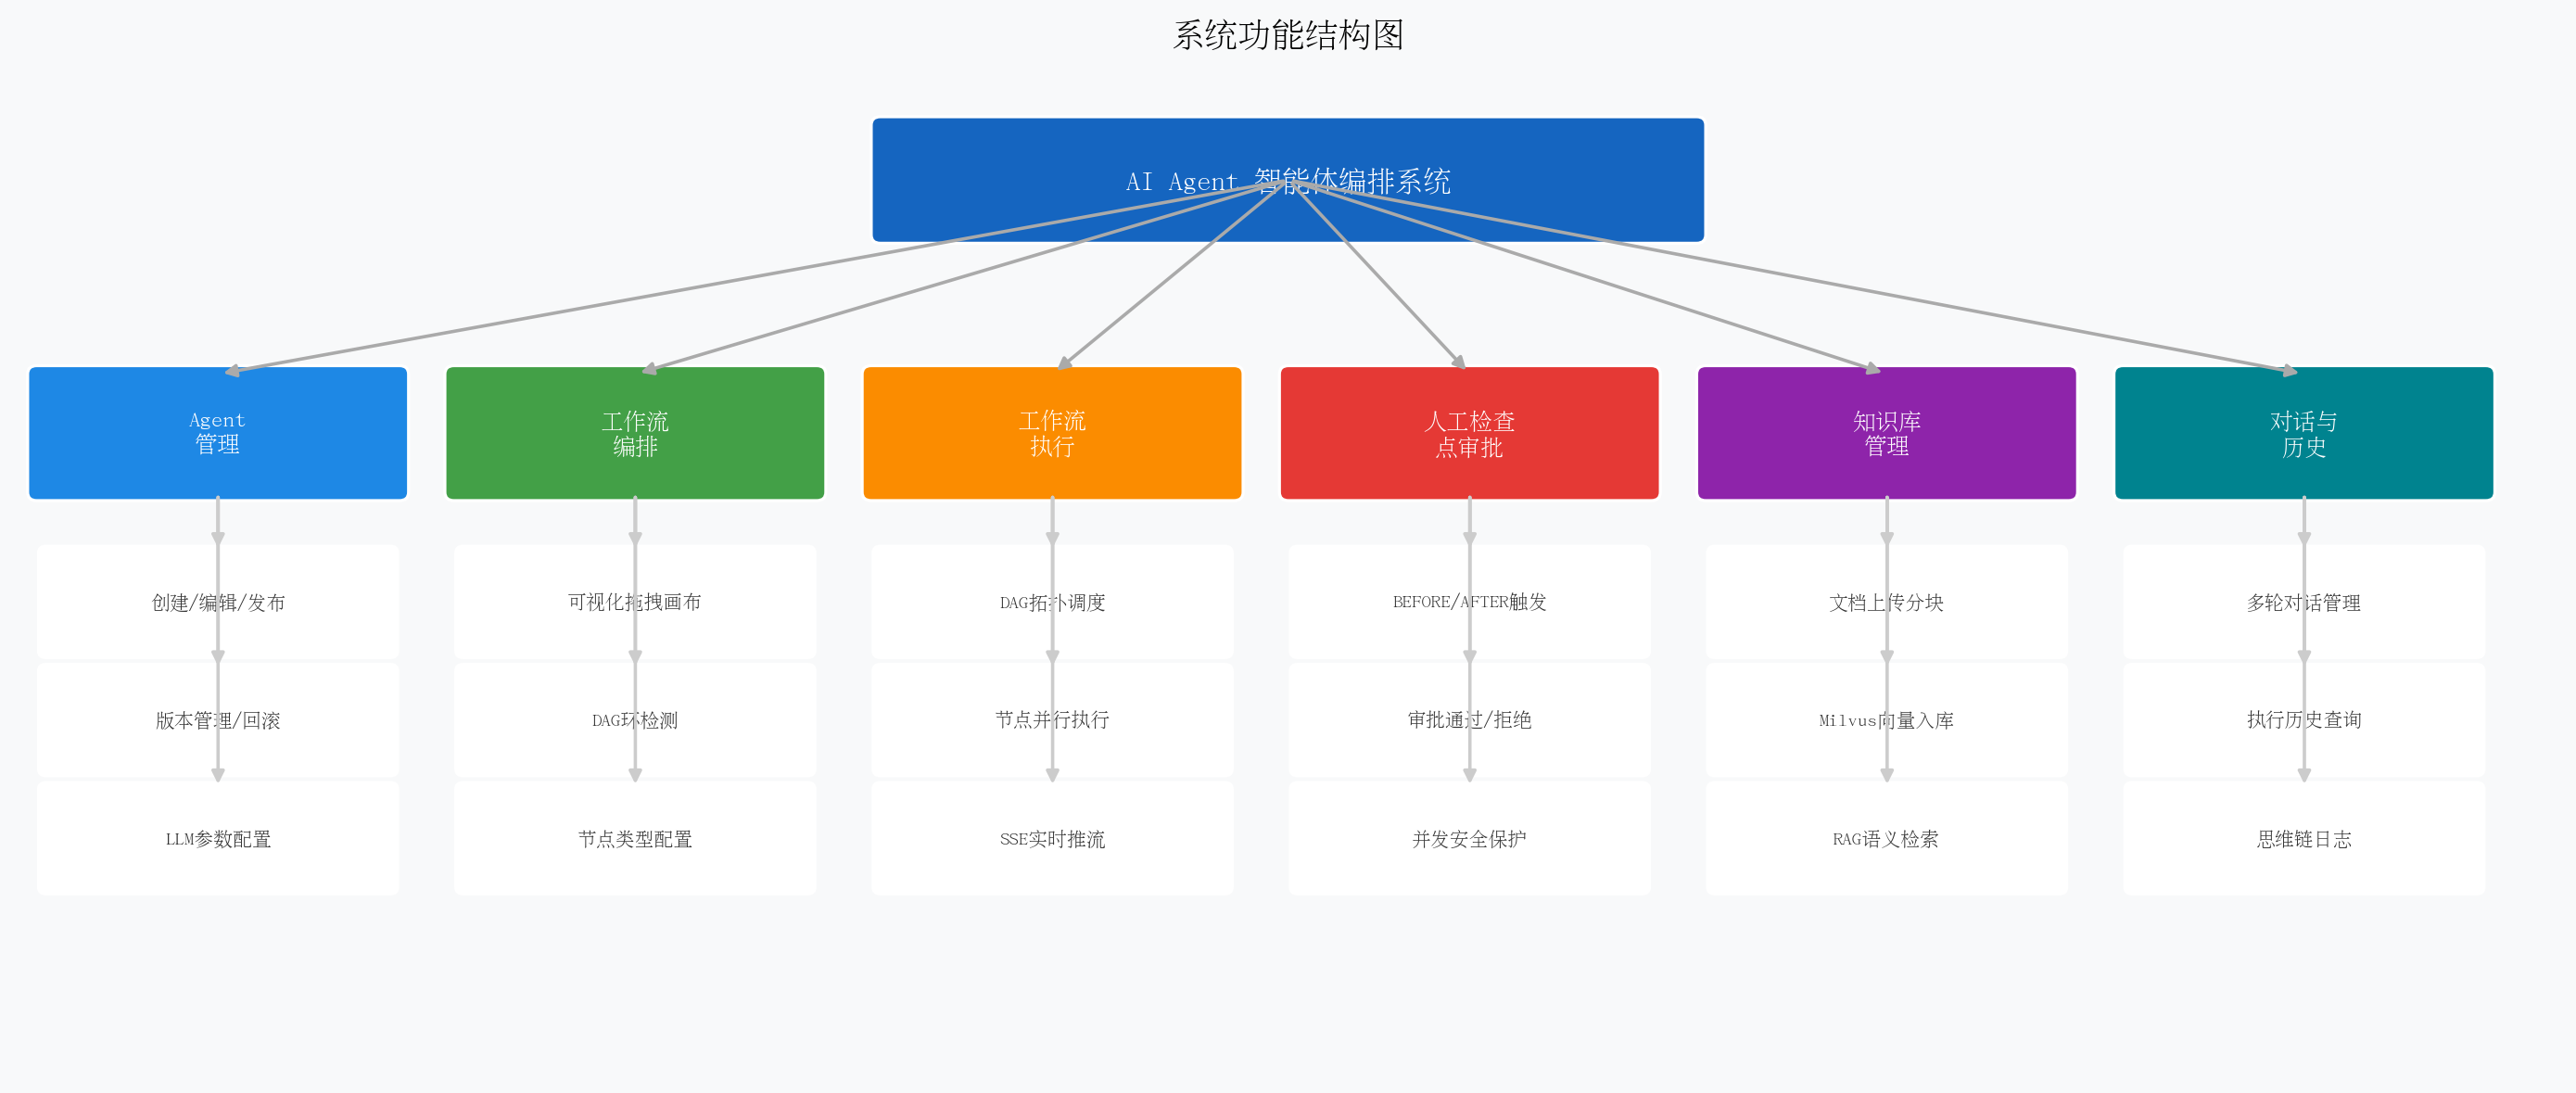
\includegraphics[width=0.98\textwidth]{figures/fig_func.png}
  \caption{系统功能结构图}
  \label{fig:func_struct}
\end{figure}

\subsection{Agent 管理与可视化编排模块}

该模块负责 Agent 的生命周期管理与可视化流程定义。
后端通过 Agent 应用服务实现创建、编辑、发布、版本查询与回滚，
每个 Agent 对应一份以 \texttt{graphJson} 形式存储的工作流定义。
前端通过 ReactFlow 画布提供拖拽式编排界面，支持节点创建、删除、参数配置和边连接，
并将画布状态统一序列化为图结构 JSON。

在发布流程中，系统会将当前草稿快照写入 \texttt{agent\_version} 表，
并更新 Agent 的已发布版本号，保证编辑中的草稿和线上执行版本相互隔离。
通过这一设计，Agent 管理模块既承担配置入口，又为运行时调度提供标准化图定义来源。

\subsection{工作流调度执行模块}

工作流执行模块以 \texttt{SchedulerService} 与 \texttt{Execution} 聚合根的协作为核心。
系统在执行开始时读取 Agent 的图定义，将 \texttt{graphJson} 反序列化为 \texttt{WorkflowGraph}，
随后初始化执行上下文、节点状态和就绪队列。

执行引擎基于 DAG 拓扑排序和事件驱动调度，
支持无依赖节点并行执行、条件分支、路径剪枝和执行状态推进。
整个执行过程通过 SSE 持续向前端推送节点启动、完成、错误和暂停恢复等事件。

执行状态机如图~\ref{fig:state_machine}~所示。

\begin{figure}[H]
  \centering
  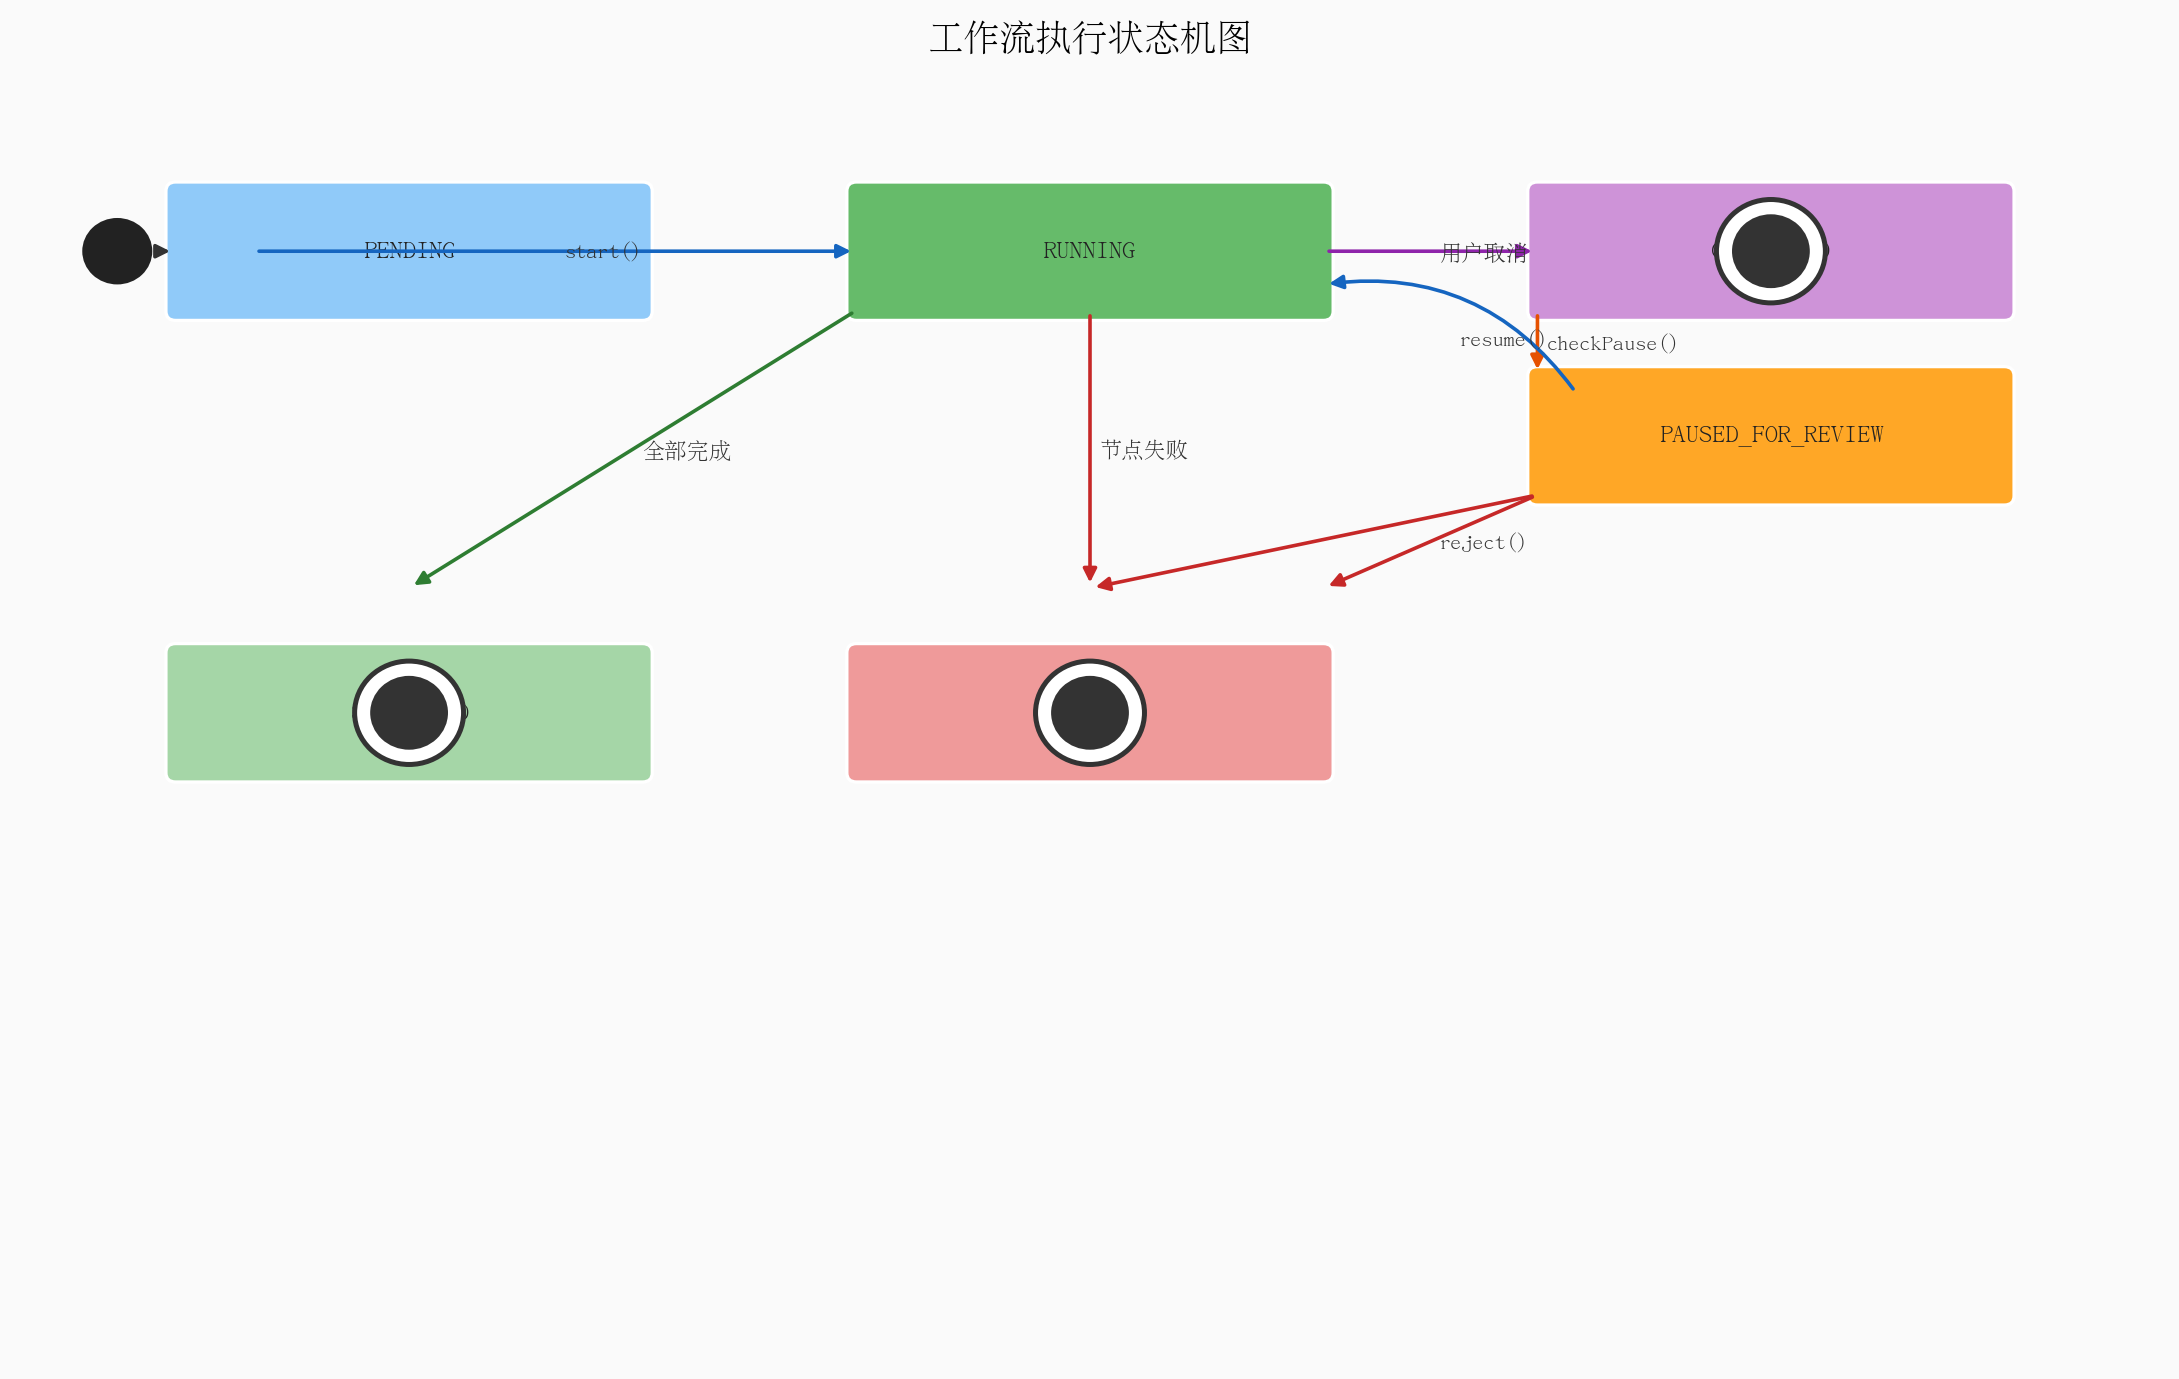
\includegraphics[width=0.88\textwidth]{figures/fig_state.png}
  \caption{工作流执行状态机}
  \label{fig:state_machine}
\end{figure}

\begin{table}[H]
  \centering
  \caption{执行状态转换说明}
  \begin{tabular}{lll}
    \toprule
    \textbf{源状态} & \textbf{目标状态} & \textbf{触发条件} \\
    \midrule
    PENDING & RUNNING & \texttt{start()} 调用成功，DAG 初始化 \\
    RUNNING & SUCCEEDED & 所有节点均完成（SUCCEEDED 或 SKIPPED） \\
    RUNNING & FAILED & 某节点执行失败 \\
    RUNNING & CANCELLED & 用户主动取消 \\
    RUNNING & PAUSED\_FOR\_REVIEW & 检查点触发，执行进入人工审核 \\
    PAUSED\_FOR\_REVIEW & RUNNING & 审批通过，\texttt{resume()} \\
    PAUSED\_FOR\_REVIEW & FAILED & 审批拒绝，\texttt{reject()} \\
    \bottomrule
  \end{tabular}
  \label{tab:state_trans}
\end{table}

\subsection{人工审核与恢复机制模块}

该模块在工作流执行链路中植入“暂停—等待—恢复/终止”的控制能力。
节点可配置人工检查点开关与触发阶段，支持 \texttt{BEFORE\_EXECUTION}
和 \texttt{AFTER\_EXECUTION} 两种模式。

设计上，系统采用 Redis 维护待审批队列，并为每个执行实例配置分布式锁；
审批人通过审批列表接口查看待处理任务，进入详情后可查看当前节点上下文、
修改中间结果并提交通过或拒绝操作。
恢复或拒绝请求均以执行版本号作为乐观锁条件，
从而防止多用户并发审批导致的状态覆盖问题。

\subsection{知识库与检索增强模块}

该模块用于为工作流中的知识节点和 LLM 节点提供外部知识支撑。
从设计上看，知识链路由数据集管理、文档管理、异步处理和语义检索四部分组成。

用户上传文档后，系统先将原始文件存入 MinIO，
再由异步处理器完成文档解析、文本分块与向量化入库。
向量数据与原始文档元信息通过 \texttt{document\_id}、\texttt{dataset\_id}、\texttt{agent\_id}
等字段建立关联，便于后续删除、筛选与语义搜索。

运行时，当知识节点或检索接口收到查询请求时，系统将查询语句向量化，
在 Milvus 中执行 Top-K 语义搜索，并将召回片段返回给后续节点作为上下文增强信息。
这一设计使知识接入链路与工作流运行链路形成完整闭环。

\subsection{用户认证与系统安全支撑模块}

该模块为整个平台提供统一的身份识别、访问控制与安全约束能力。
系统支持邮箱注册、登录、找回密码和 JWT 令牌认证，
其中验证码发送、密码强度校验、密码哈希存储与登录失败限制均在认证领域服务中实现。

认证成功后，接口层在请求上下文中解析用户身份，
业务模块据此执行 Agent 所有权校验、知识库访问控制、审批操作记录等逻辑。
因此，用户认证与系统安全并不是孤立模块，而是贯穿其他四个业务模块的基础支撑层。

\section{核心数据流设计}

为体现五个模块之间的衔接关系，系统在设计上形成了如下三条关键数据流。

\subsection{Agent 编排到运行时执行的数据流}

用户在前端画布完成 Agent 编排后，画布中的节点和边会被序列化为 \texttt{graphJson}。
当用户点击保存时，后端执行图结构校验并将其保存为草稿；
点击发布后，系统生成版本快照并固化为可执行版本。
运行时，调度器根据 Agent ID 与版本号读取对应的图定义，
再将 JSON 反序列化为 \texttt{WorkflowGraph}，作为 \texttt{Execution} 聚合根的输入。

\subsection{知识接入到检索增强的数据流}

用户上传文档后，接口层将文件流和分块配置传递给知识应用服务；
应用服务先进行文件校验并上传到 MinIO，再创建文档记录并触发异步处理器。
异步处理器下载原始文件，解析为文本段落，调用文本切分器生成多个文本块，
随后通过向量存储接口将其写入 Milvus。
执行期收到查询时，系统以相同的语义向量检索方式召回相关片段，
再将其注入工作流上下文供后续节点使用。

\subsection{认证安全到业务访问控制的数据流}

用户注册或登录成功后，系统签发 JWT 令牌，前端在后续请求中统一携带。
接口层解析令牌并写入当前用户上下文，应用服务据此进行资源所有权校验。
例如 Agent 更新必须校验 Agent 是否属于当前用户，
知识文档上传必须校验数据集归属，人工审批记录必须保存当前审批人 ID。
这一数据流保证了平台各模块均运行在统一的认证与授权边界内。

\section{数据库设计}

系统采用 MySQL 8.0 存储业务数据，核心数据表清单如表~\ref{tab:db_tables}~所示。

\begin{table}[H]
  \centering
  \caption{核心数据表清单}
  \label{tab:db_tables}
  \begin{tabular}{lll}
    \toprule
    \textbf{表名} & \textbf{所属模块} & \textbf{用途} \\
    \midrule
    \texttt{agent} & Agent 管理 & Agent 基本信息与草稿图定义 \\
    \texttt{agent\_version} & Agent 管理 & Agent 版本快照（含 graphJson） \\
    \texttt{workflow\_execution} & 工作流执行 & 执行记录（状态/暂停节点/版本号/上下文） \\
    \texttt{workflow\_execution\_node} & 工作流执行 & 节点执行日志（输入/输出/耗时） \\
    \texttt{workflow\_human\_review\_record} & 人工审核 & 审批记录（审批人/决策/修改内容/原因） \\
    \texttt{knowledge\_dataset} & 知识库 & 知识数据集基本信息 \\
    \texttt{knowledge\_document} & 知识库 & 文档记录、处理状态和分块配置 \\
    \texttt{user} & 用户认证 & 用户账户信息与密码哈希 \\
    \texttt{chat\_conversation} & 对话 & 会话记录 \\
    \texttt{chat\_message} & 对话 & 消息记录与短期上下文 \\
    \bottomrule
  \end{tabular}
\end{table}

表~\ref{tab:execution_schema}~列出了 \texttt{workflow\_execution} 表的关键字段设计，
该表是工作流执行状态的核心持久化存储。

\begin{table}[H]
  \centering
  \caption{workflow\_execution 关键字段设计}
  \label{tab:execution_schema}
  \begin{tabular}{llll}
    \toprule
    \textbf{字段名} & \textbf{类型} & \textbf{说明} & \textbf{备注} \\
    \midrule
    execution\_id & VARCHAR & 执行唯一标识 & 主键，UUID \\
    agent\_id & BIGINT & 所属 Agent & 外键 \\
    user\_id & BIGINT & 触发用户 & 外键 \\
    status & VARCHAR & 执行状态枚举 & 见状态机表 \\
    paused\_node\_id & VARCHAR & 当前暂停节点 & 暂停时设置，恢复后清空 \\
    paused\_phase & VARCHAR & 暂停阶段 & BEFORE / AFTER\_EXECUTION \\
    version & INT & 乐观锁版本号 & 每次状态变更自增 \\
    node\_statuses & JSON & 各节点状态 Map & PENDING/RUNNING/SUCCEEDED/FAILED/SKIPPED \\
    context & JSON & 执行上下文快照 & 含 inputs/nodeOutputs/chatHistory/检索结果 \\
    reviewed\_nodes & JSON & 已审批节点集合 & 防止 resume 后重复暂停 \\
    \bottomrule
  \end{tabular}
\end{table}

表~\ref{tab:review_schema}~列出了 \texttt{workflow\_human\_review\_record} 表的关键字段，
该表记录所有人工审批操作，用于事后审计和合规查询。

\begin{table}[H]
  \centering
  \caption{workflow\_human\_review\_record 关键字段设计}
  \label{tab:review_schema}
  \begin{tabular}{llll}
    \toprule
    \textbf{字段名} & \textbf{类型} & \textbf{说明} & \textbf{备注} \\
    \midrule
    id & BIGINT & 主键 & 自增 \\
    execution\_id & VARCHAR & 关联执行 ID & 外键 \\
    node\_id & VARCHAR & 审批节点 ID & 与 DAG 节点一致 \\
    reviewer\_id & BIGINT & 审批人用户 ID & 外键 \\
    decision & VARCHAR & 审批决策 & APPROVE / REJECT \\
    trigger\_phase & VARCHAR & 触发阶段 & BEFORE / AFTER\_EXECUTION \\
    original\_data & JSON & 节点原始输出 & reject 时记录 \\
    modified\_data & JSON & 审批人修改内容 & approve + edits 时记录 \\
    comment & VARCHAR & 审批意见/拒绝原因 & 可为空 \\
    reviewed\_at & DATETIME & 审批时间 & NOT NULL \\
    \bottomrule
  \end{tabular}
\end{table}

表~\ref{tab:knowledge_schema}~列出了知识文档表的关键字段设计。

\begin{table}[H]
  \centering
  \caption{knowledge\_document 关键字段设计}
  \label{tab:knowledge_schema}
  \begin{tabular}{llll}
    \toprule
    \textbf{字段名} & \textbf{类型} & \textbf{说明} & \textbf{备注} \\
    \midrule
    document\_id & VARCHAR & 文档唯一标识 & 主键 \\
    dataset\_id & VARCHAR & 所属数据集 & 外键 \\
    filename & VARCHAR & 原始文件名 & 上传时写入 \\
    file\_url & VARCHAR & 对象存储地址 & MinIO 文件路径 \\
    status & VARCHAR & 处理状态 & PENDING/PROCESSING/COMPLETED/FAILED \\
    total\_chunks\_count & INT & 分块总数 & 处理完成后更新 \\
    chunking\_config & JSON & 分块配置 & 固定分块/语义分块参数 \\
    \bottomrule
  \end{tabular}
\end{table}

\section{技术选型}

表~\ref{tab:tech_stack}~列出了系统各层次的技术选型及选择依据。

\begin{table}[H]
  \centering
  \caption{系统技术栈选型}
  \label{tab:tech_stack}
  \begin{tabular}{llp{5cm}}
    \toprule
    \textbf{类别} & \textbf{技术} & \textbf{选型依据} \\
    \midrule
    运行时 & Java 21 & 虚拟线程支持，IO 密集场景并发能力显著提升 \\
    后端框架 & Spring Boot 3.x & 依赖注入、自动配置、生态成熟 \\
    AI 集成 & Spring AI & Spring 官方 LLM 接入框架，统一 ChatClient 接口 \\
    ORM & MyBatis Plus & 灵活 SQL 控制，适合工作流复杂查询 \\
    关系型数据库 & MySQL 8.0 & 业务数据持久化，JSON 字段存储上下文 \\
    缓存 / 分布式锁 & Redis + Redisson & 待审批队列、分布式锁、热数据缓存 \\
    向量数据库 & Milvus 2.3 & 高性能语义向量检索，适合知识增强场景 \\
    对象存储 & MinIO & 存储原始文档文件，便于异步处理与回溯 \\
    实时推流 & SSE & 长连接、浏览器原生支持、无需额外协议 \\
    前端框架 & React + TypeScript & 组件化开发，类型安全 \\
    流程画布 & ReactFlow & 成熟的 DAG 可视化编排库 \\
    容器化 & Docker Compose & 一键启动所有依赖服务，环境一致 \\
    \bottomrule
  \end{tabular}
\end{table}

\section{本章小结}

本章完成了 AI Agent 智能体编排系统的概要设计。
首先确定了基于 DDD 的四层架构（接口层 / 应用层 / 领域层 / 基础设施层）的整体结构，
随后围绕 Agent 管理与可视化编排、工作流调度执行、人工审核与恢复机制、
知识库与检索增强、用户认证与系统安全支撑五个模块进行了职责划分，
并补充了 Agent 编排到运行时执行、知识接入到检索增强、认证安全到访问控制三条核心数据流设计。
最后，本文给出了关键业务表结构与技术选型依据，
为第四章的详细实现提供了完整的设计蓝图。
